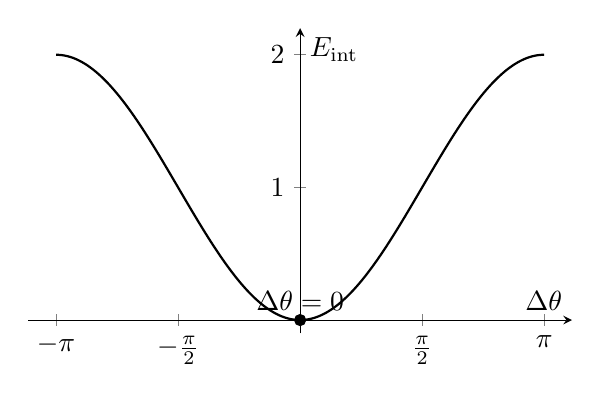
\begin{tikzpicture}
  \begin{axis}[
      width=0.7\textwidth,
      height=0.45\textwidth,
      axis lines=middle,
      xlabel={$\Delta\theta$},
      ylabel={$E_{\mathrm{int}}$},
      xmin=-3.5, xmax=3.5,
      ymin=-0.1, ymax=2.2,
      xtick={-3.1416,-1.5708,0,1.5708,3.1416},
      xticklabels={$-\pi$, $-\frac{\pi}{2}$, $0$, $\frac{\pi}{2}$, $\pi$},
      ytick={0,1,2},
      domain=-3.1416:3.1416,
      samples=200,
      smooth
  ]
    \addplot[thick] {1 - cos(deg(x))};
    \addplot[only marks, mark=*, mark size=2pt] coordinates {(0,0)};
    \node[anchor=south] at (axis cs:0,0) {$\Delta\theta=0$};
  \end{axis}
\end{tikzpicture}
